\documentclass[a4paper]{article}

\usepackage[a4paper, top=8mm, bottom=8mm, left=8mm, right=8mm]{geometry}
\usepackage{float}
\usepackage{graphicx}

\usepackage{polyglossia}
\setdefaultlanguage[babelshorthands=true]{russian}
\setotherlanguage{english}

\usepackage{fontspec}
\setmainfont{FreeSerif}
\newfontfamily{\russianfonttt}[Scale=0.7]{DejaVuSansMono}

\usepackage[tiny, compact]{titlesec}

\usepackage{titling}
\setlength{\droptitle}{-1cm}
\pretitle{\begin{center}\begin{bfseries}\Large}
\posttitle{\par\end{bfseries}\end{center}}
\preauthor{\begin{center}\normalsize}
\postauthor{\par\end{center}\vspace{-1.8cm}}

\usepackage{hyperref}
\usepackage{bookmark}
\usepackage{csquotes}
\usepackage{booktabs}
\usepackage{multirow}

\title{LaMaGraph: Разреженные матрицы на F\#}

\author{Брулевич Никита Петрович}

\date{}

\begin{document}

\maketitle

\begin{flushright}
    Группа: \emph{2025.Б-73-мм}
    
    Кафедра: \emph{кафедра системного программирования}
    
    Научный руководитель: \emph{Григорьев Семён Вячеславович}
    
    Номер семестра практики: \emph{2}
\end{flushright}

\section{Постановка задачи}

Работа выполняется в рамках проекта \textbf{LamaGraph} (Lambdas, Matrices and Graphs), нацеленного на разработку прототипа быстрого вычислителя для разреженной линейной алгебры, реализованного в функциональной парадигме программирования на языке F\#.

Одной из ключевых частей проекта является библиотека \textbf{QTreeFSharp} для работы с разреженными матрицами и векторами на языке F\#, реализованная на деревьях квадрантов (quadtree).

\textbf{Целью работы} является реализация и оптимизация следующих операций над разреженными матрицами и векторами:
\begin{itemize}
    \item Редукция (свёртка) строк и столбцов матриц -- \texttt{reduceRows}, \texttt{reduceCols}
    \item Срез (slice) векторов и матриц
    \item Произведение Кронекера (kroneckerProduct)
    \item Преобразование каждого ненулевого элемента матрицы (map)
\end{itemize}

Данные операции необходимы для реализации графовых алгоритмов и оптимизации работы матричных алгоритмов в рамках прототипа вычислителя LamaGraph.

\section{Описание предлагаемого решения}

\subsection{Структуры данных}

Разреженные векторы реализованы на бинарном дереве (\texttt{btree}), где листья содержат \texttt{UserValue} или \texttt{Dummy}. Размер дерева округляется до ближайшей степени двойки.

Разреженные матрицы реализованы на дереве квадрантов (\texttt{qtree}) с четырьмя подузлами (NW, NE, SW, SE), что позволяет рекурсивно делить матрицу на квадранты.

\subsection{Реализованные операции}

\begin{itemize}
    \item \texttt{reduceRows}, \texttt{reduceCols} -- свёртка матрицы в вектор с использованием заданной бинарной операции по строкам и по столбцам соответственно
    \item \texttt{slice} -- выделение подматрицы/подвектора по заданным границам
    \item \texttt{kroneckerProduct} -- произведение Кронекера двух матриц
    \item \texttt{map} -- применение функции к каждому ненулевому элементу матрицы
\end{itemize}

Также была изменена сигнатура функции fromCoordinateList в Matrix.fs и Vector.fs, добавлена валидация аргументов.

Дополнительно проведено сравнение двух способов реализации \texttt{reduceCols}:
\begin{enumerate}
    \item Прямой обход по столбцам (оригинальная реализация)
    \item Транспонирование матрицы с последующей свёрткой по строкам (альтернативный подход с учётом уже реализованной в проекте функции transpose).
\end{enumerate}

\subsection{Тестирование}

Для каждой из новых реализованных функций написаны Unit-тесты:
\begin{itemize}
    \item \texttt{Vector.slice} -- 11 тестов
    \item \texttt{Matrix.map} -- 6 тестов
    \item \texttt{Matrix.slice} -- 22 теста
    \item \texttt{Matrix.reduceRows} -- 7 тестов
    \item \texttt{Matrix.reduceCols} -- 7 тестов
    \item \texttt{Matrix.kroneckerProduct} -- 13 тестов
\end{itemize}
А также добавлены отсутствующие тесты на уже имевшиеся функции - 17 тестов.

\section{Эксперименты}

\subsection{Методология}

Бенчмарки проводились с использованием \texttt{BenchmarkDotNet v0.15.8} на виртуальной машине с 4GB RAM. Для каждого теста измерялись среднее время выполнения (Mean), стандартное отклонение (StdDev) и объём аллоцированной памяти (Allocated).

Использовались синтетические матрицы следующих типов:
\begin{itemize}
    \item \textbf{Sparse} --- разреженные матрицы со случайными значениями (плотность 1\%, 5\%, 10\%)
    \item \textbf{DenseUniform} --- плотные матрицы с единичными значениями (оптимальный случай)
    \item \textbf{DenseRandom} --- плотные матрицы со случайными значениями (использовалось в экспериментах над reduceCols и reduceRows)
\end{itemize}

\subsection{Результаты}

\subsubsection{ReduceRows и ReduceCols}

\begin{table}[H]
\centering
\caption{Результаты Reduce бенчмарков}
\begin{tabular}{lccc}
\toprule
Метод & Размер & Время (Mean) & Аллокации \\
\midrule
\multicolumn{4}{c}{\textbf{Sparse (разреженные, случайные)}} \\
\midrule
ReduceRows\_SparseSmall & 32×32 & 64.2 μs & 67.6 KB \\
ReduceCols\_SparseSmall & 32×32 & 65.7 μs & 72.7 KB \\
ReduceRows\_SparseMedium & 256×256 & 1.73 ms & 1.27 MB \\
ReduceCols\_SparseMedium & 256×256 & 1.87 ms & 1.35 MB \\
ReduceRows\_SparseLarge & 1024×1024 & 9.31 ms & 4.59 MB \\
ReduceCols\_SparseLarge & 1024×1024 & 10.16 ms & 4.97 MB \\
\midrule
\multicolumn{4}{c}{\textbf{DenseUniform (плотные, все 1.0)}} \\
\midrule
ReduceRows\_DenseUniformSmall & 32×32 & 255.6 μs & 308 KB \\
ReduceCols\_DenseUniformSmall & 32×32 & 264.5 μs & 313 KB \\
ReduceRows\_DenseUniformMedium & 256×256 & 56.7 ms & 17.6 MB \\
ReduceCols\_DenseUniformMedium & 256×256 & 72.4 ms & 17.6 MB \\
ReduceRows\_DenseUniformLarge & 1024×1024 & 856 ms & 276 MB \\
ReduceCols\_DenseUniformLarge & 1024×1024 & 1137 ms & 277 MB \\
\midrule
\multicolumn{4}{c}{\textbf{DenseRandom (плотные, случайные)}} \\
\midrule
ReduceRows\_DenseRandomSmall & 32×32 & 277.6 μs & 308 KB \\
ReduceCols\_DenseRandomSmall & 32×32 & 293.2 μs & 312 KB \\
ReduceRows\_DenseRandomMedium & 256×256 & 77.9 ms & 17.6 MB \\
ReduceCols\_DenseRandomMedium & 256×256 & 74.6 ms & 17.6 MB \\
ReduceRows\_DenseRandomLarge & 1024×1024 & 1072 ms & 276 MB \\
ReduceCols\_DenseRandomLarge & 1024×1024 & 1106 ms & 277 MB \\
\bottomrule
\end{tabular}
\end{table}

\subsubsection{Сравнение reduceCols и reduceCols как transpose + reduceRows}

\begin{table}[H]
\centering
\small
\caption{Сравнение прямой реализации reduceCols и реализации через транспонирование}
\begin{tabular}{lcccccc}
\toprule
\multirow{2}{*}{Метод} & \multirow{2}{*}{Размер} & \multicolumn{2}{c}{Время (Mean)} & \multicolumn{2}{c}{Аллокации} & \multirow{2}{*}{Разница по времени} \\
\cline{3-6}
& & Оригинал & Транспонирование & Оригинал & Транспонирование & \\
\midrule
ReduceCols\_SparseSmall & 32×32 & 66.5 μs & 78.5 μs & 72.7 KB & 75.0 KB & +18\% \\
ReduceCols\_DenseSmall & 32×32 & 265 μs & 261 μs & 313 KB & 310 KB & -1.5\% \\
ReduceCols\_SparseMedium & 256×256 & 1.84 ms & 2.78 ms & 1.35 MB & 1.40 MB & +51\% \\
ReduceCols\_DenseMedium & 256×256 & 64.8 ms & 57.5 ms & 17.6 MB & 17.6 MB & \textbf{-11\%} \\
ReduceCols\_SparseLarge & 1024×1024 & 9.89 ms & 19.5 ms & 4.97 MB & 5.10 MB & +97\% \\
ReduceCols\_DenseLarge & 1024×1024 & 1.14 s & 0.89 s & 277 MB & 277 MB & \textbf{-22\%} \\
\bottomrule
\end{tabular}
\end{table}

\begin{figure}[H]
\centering
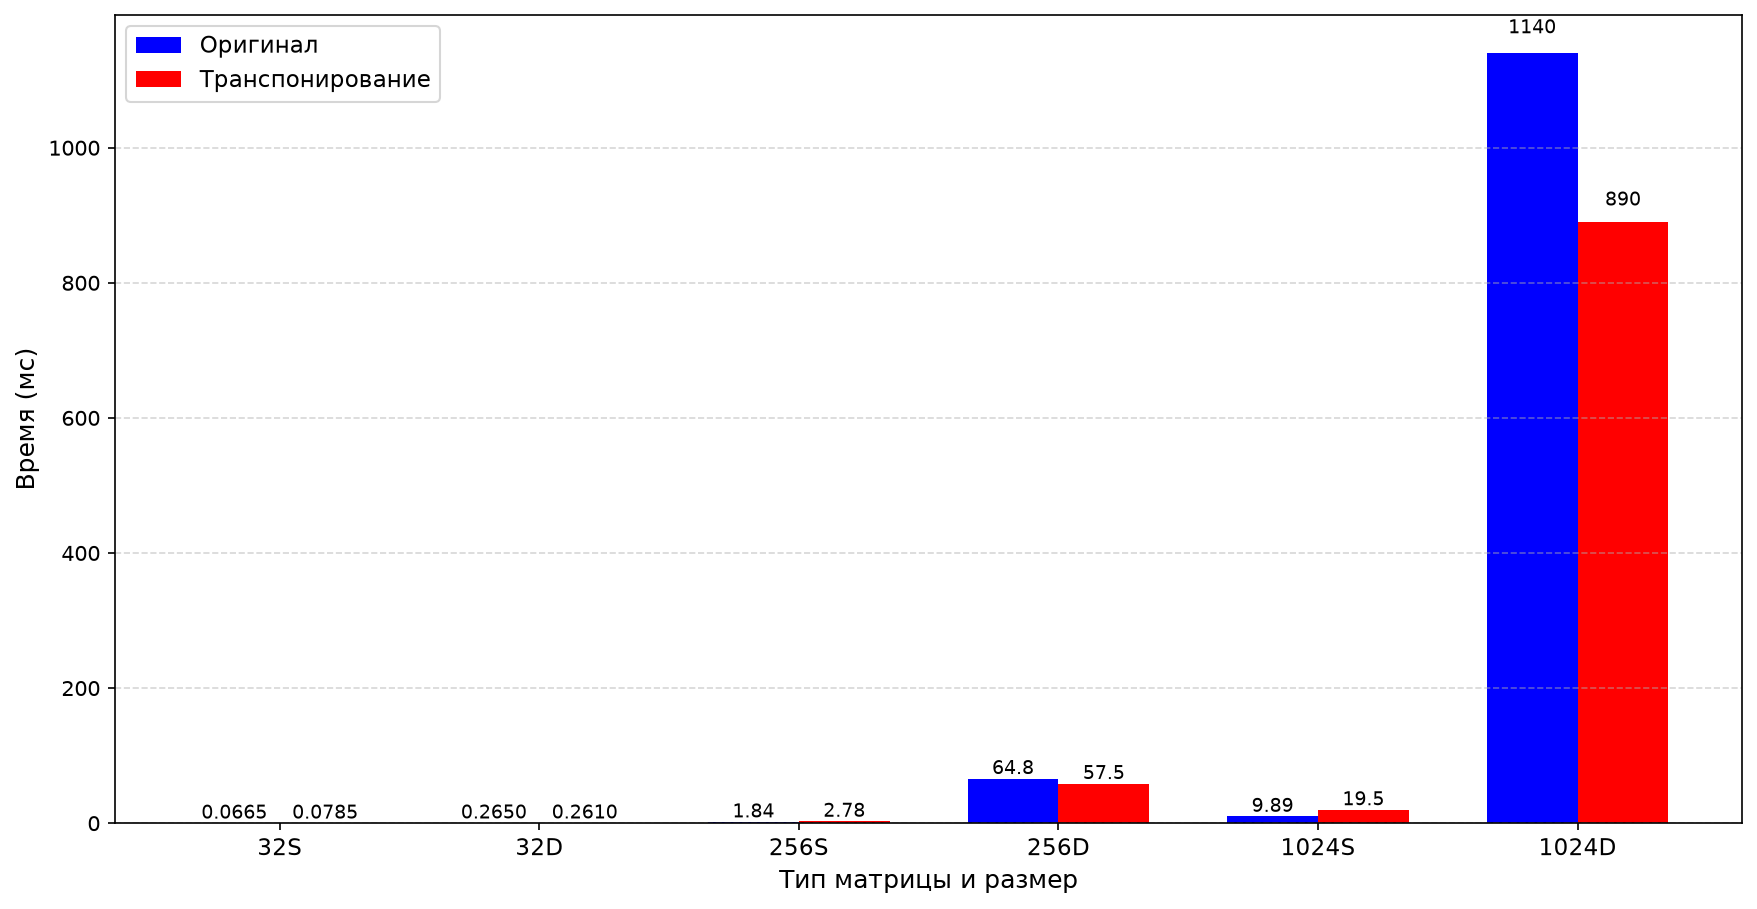
\includegraphics[width=0.85\textwidth]{images/time_comparison.png}
\caption{Сравнение времени выполнения оригинального reduceCols и реализации через транспонирование}
\label{fig:reducecols_time}
\end{figure}

\begin{figure}[H]
\centering
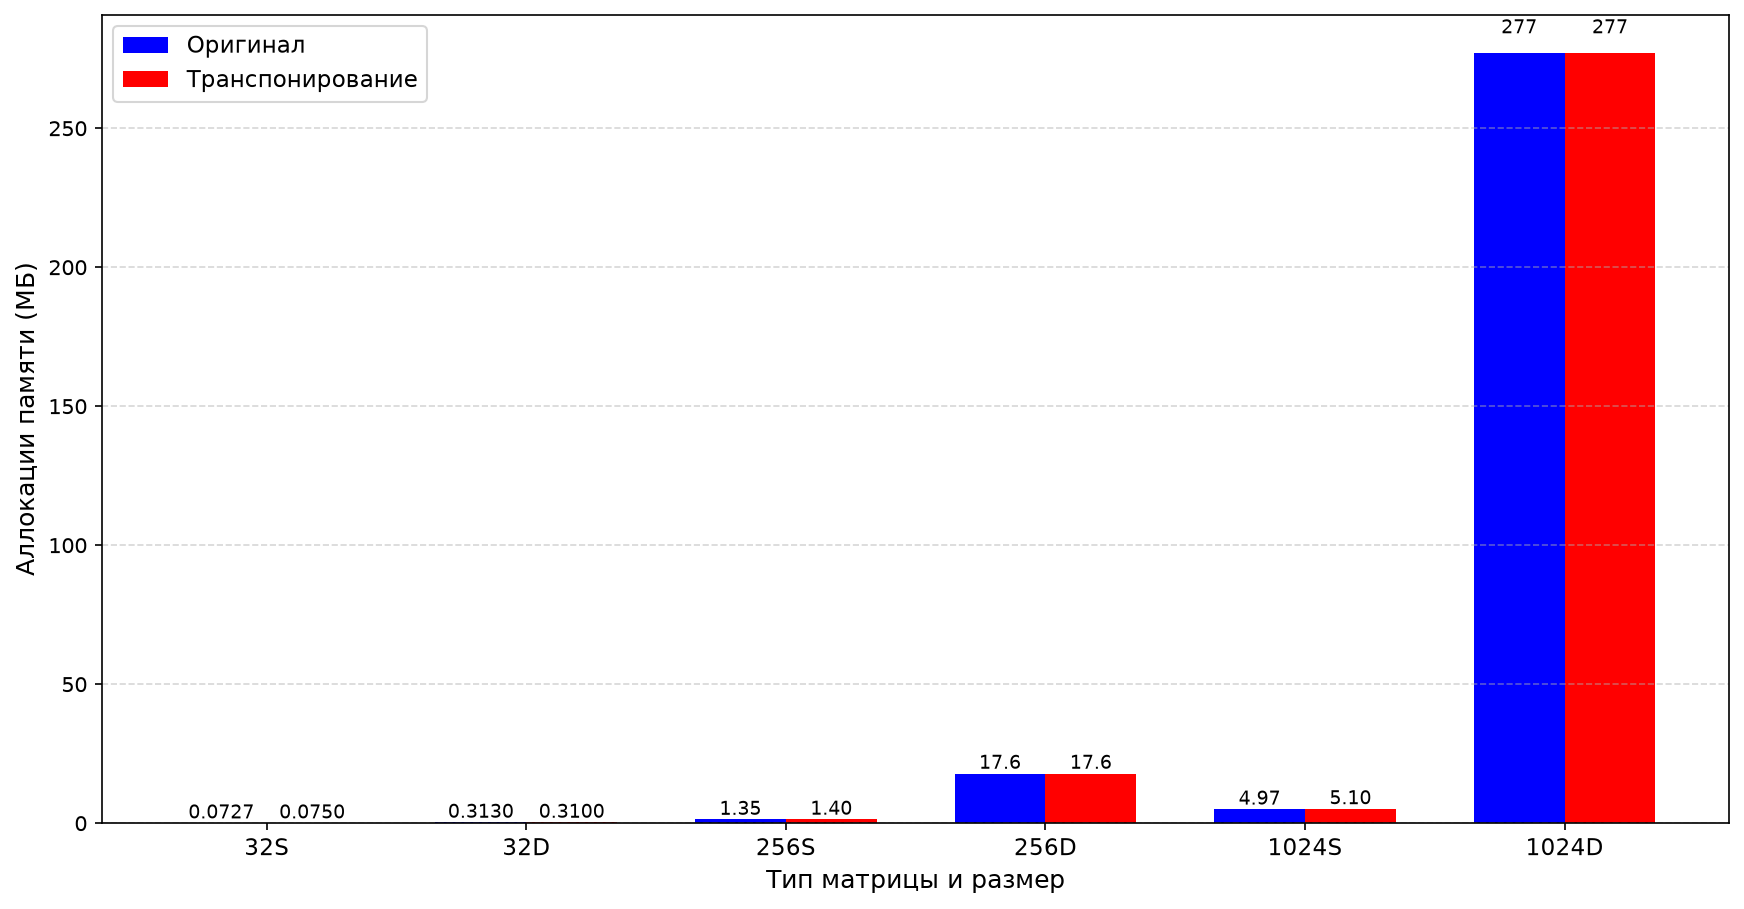
\includegraphics[width=0.85\textwidth]{images/memory_comparison.png}
\caption{Сравнение аллокаций памяти оригинального reduceCols и реализации через транспонирование}
\label{fig:reducecols_memory}
\end{figure}

На плотных матрицах реализация через транспонирование оказывается быстрее на 10-22\% благодаря лучшей кэш-локальности. На разреженных матрицах, напротив, прямой обход по столбцам оказывается быстрее на 18-97\%.

\subsubsection{Slice для векторов}

\begin{table}[H]
\centering
\caption{Результаты VectorSlice (срез середины)}
\begin{tabular}{lccc}
\toprule
Метод & Размер & Время (Mean) & Аллокации \\
\midrule
Slice\_SparseSmall & 32 & 2.6 μs & 3.8 KB \\
Slice\_DenseSmall & 32 & 2.8 μs & 4.5 KB \\
Slice\_SparseMedium & 256 & 29.7 μs & 42.5 KB \\
Slice\_DenseMedium & 256 & 31.6 μs & 46.3 KB \\
Slice\_SparseLarge & 1024 & 181 μs & 212 KB \\
Slice\_DenseLarge & 1024 & 178 μs & 216 KB \\
\bottomrule
\end{tabular}
\end{table}

\subsubsection{Slice для матриц}

\begin{table}[H]
\centering
\caption{Результаты MatrixSlice (срез середины)}
\begin{tabular}{lccc}
\toprule
Метод & Размер & Время (Mean) & Аллокации \\
\midrule
MatrixSlice\_SparseSmall & 32×32 & 68.8 μs & 68 KB \\
MatrixSlice\_DenseSmall & 32×32 & 53.3 μs & 77 KB \\
MatrixSlice\_SparseMedium & 256×256 & 14.0 ms & 6.9 MB \\
MatrixSlice\_DenseMedium & 256×256 & 15.0 ms & 7.2 MB \\
MatrixSlice\_SparseLarge & 1024×1024 & 285 ms & 138 MB \\
MatrixSlice\_DenseLarge & 1024×1024 & 302 ms & 139 MB \\
\bottomrule
\end{tabular}
\end{table}

\subsubsection{Произведение Кронекера}

\begin{table}[H]
\centering
\caption{Результаты KroneckerProduct}
\begin{tabular}{lccc}
\toprule
Метод & Исходный размер & Время (Mean) & Аллокации \\
\midrule
Kronecker\_SparseSmall & 8×8 & 92.1 μs & 86 KB \\
Kronecker\_DenseSmall & 8×8 & 2.31 ms & 1.5 MB \\
Kronecker\_SparseMedium & 16×16 & 1.20 ms & 229 KB \\
Kronecker\_DenseMedium & 16×16 & 114 ms & 31 MB \\
Kronecker\_SparseLarge & 32×32 & 6.22 ms & 112 KB \\
Kronecker\_DenseLarge & 32×32 & 1.29 s & 576 MB \\
\bottomrule
\end{tabular}
\end{table}

\subsection{Выводы из экспериментов}

\begin{enumerate}
    \item \textbf{Редукция матриц (reduceRows, reduceCols)}: разреженные матрицы демонстрируют преимущество над плотными во всех размерах. На малых матрицах (32×32) выигрыш составляет 3-4 раза (64-66 μs против 256-293 μs), на средних (256×256) -- 30-40 раз (1.7-1.9 ms против 56-78 ms), на больших (1024×1024) -- до 120 раз (9-10 ms против 856-1137 ms). Аллокации памяти также отличаются в 4, 15 и 60 раз соответственно. Результаты времени выполнения для плотных матриц с единичными и случайными значениями (DenseUniform и DenseRandom) близки, разница не превышает 25\%, разница объёма аллоцированной памяти - не более 2\%.

    \item \textbf{Сравнение реализаций reduceCols}: транспонирование эффективнее на плотных матрицах (ускорение растёт с размером: 1.5\%, 11\%, 22\%), но проигрывает на разреженных (замедление 18\%, 51\%, 97\%). Это объясняется лучшей кэш-локальностью при последовательном обходе строк после транспонирования.

    \item \textbf{Срез (slice)}: на всех размерах производительность для разреженных и плотных матриц/векторов остаётся сопоставимой (разница не превышает 10-15\%).

    \item \textbf{Произведение Кронекера}: выигрыш разреженных матриц над плотными растёт с размером. Для матриц 8×8 разреженная быстрее в 25 раз (92 μs против 2.3 ms), для 16×16 -- в 95 раз (1.2 ms против 114 ms), для 32×32 -- в 200 раз (6.2 ms против 1.29 с). Аллокации памяти различаются ещё сильнее: 86 KB против 1.5 MB (8×8), 229 KB против 31 MB (16×16), 112 KB против 576 MB (32×32). Соотношение по памяти достигает 5000 раз на максимальном размере.
\end{enumerate}

\section{Заключение}
В ходе выполнения работы получены следующие результаты:

\begin{itemize}
    \item Реализованы и оптимизированы операции \texttt{reduceRows}, \texttt{reduceCols}, \texttt{slice}, \texttt{kroneckerProduct}, \texttt{map} для разреженных матриц и векторов.
    \item Проведено сравнение двух подходов к реализации \texttt{reduceCols}, показавшее преимущество транспонирования на плотных матрицах.
    \item Выполнены бенчмарки для реализованных функций на плотных и разреженных векторах и матрицах разного размера.
    \item Полученные результаты задокументированы и могут быть использованы для дальнейшей оптимизации графовых алгоритмов и работы с матрицами.
\end{itemize}

\section{Источники}
\begin{thebibliography}{99}
\bibitem{qtreefsharp} Исходный код проекта QTreeFSharp. URL: \url{https://github.com/Lamagraph/QTreeFSharp}

\bibitem{benchmarkdotnet} Официальная документация инструмента профилирования BenchmarkDotNet. URL: \url{https://benchmarkdotnet.org/}

\bibitem{fsharpdocs} Документация по языку F\#. URL: \url{https://learn.microsoft.com/ru-ru/dotnet/fsharp/}
\end{thebibliography}

\section{Репозиторий}
\url{https://github.com/Brulevich-Nikita/QTreeFSharp1}

\end{document}
